\documentclass{vkr}
\usepackage[english, russian]{babel} % переносы
\usepackage{graphicx} % для вставки картинок
\graphicspath{{images/}} % путь к изображениям
\usepackage[hidelinks]{hyperref}
\usepackage{float} % определяет метод H для рисунка с переносом на следующую страницу, ели не помещается
\usepackage{pdflscape}
\addto{\captionsrussian}{\renewcommand{\refname}{СПИСОК ИСПОЛЬЗОВАННЫХ ИСТОЧНИКОВ}}
\usepackage{xltabular} % для вставки таблиц
\usepackage{makecell}
\renewcommand\theadfont{} % шрифт в /thead
\usepackage{array} % для определения новых типов столбцов таблиц
\newcolumntype{T}{>{\centering\arraybackslash}X} % новый тип столбца T - автоматическая ширина столбца с выравниванием по центру
\newcolumntype{R}{>{\raggedleft\arraybackslash}X} % новый тип столбца R - автоматическая ширина столбца с выравниванием по правому краю
\newcolumntype{C}[1]{>{\centering\let\newline\\\arraybackslash\hspace{0pt}}m{#1}} % новый тип столбца C - фиксированная ширина столбца с выравниванием по центру
\newcolumntype{r}[1]{>{\raggedleft\arraybackslash}p{#1}} % новый тип столбца r - фиксированная ширина столбца с выравниванием по правому краю
\newcommand{\centrow}{\centering\arraybackslash} % командой \centrow можно центрировать одну ячейку (заголовок) в столбце типа X или p, оставив в оcтальных ячейках другой тип выравнивания
\newcommand{\finishhead}{\endhead\hline\endlastfoot}
\newcommand{\continuecaption}[1]{\captionsetup{labelformat=empty} \caption[]{#1}\\ \hline }
\usepackage{etoolbox}
\AtBeginEnvironment{xltabular}{\refstepcounter{tablecnt}} % подсчет таблиц xltabular, обычные таблицы подсчитываются в классе

\usepackage[tableposition=top]{caption} % подпись таблицы вверху
\captionsetup{strut=off}
\setlength{\intextsep}{0pt} % Vertical space above & below [h] floats
\setlength{\textfloatsep}{0pt} % Vertical space below (above) [t] ([b]) floats
\DeclareCaptionLabelFormat{gostfigure}{Рисунок #2} %подпись рисунка
\DeclareCaptionLabelFormat{gosttable}{Таблица #2} %подпись таблицы
\DeclareCaptionLabelSeparator{gost}{~--~} %разделитель в рисунках и таблицах
\captionsetup{labelsep=gost}
\captionsetup[figure]{aboveskip=10pt,belowskip=4mm,justification=centering,labelformat=gostfigure} % настройка подписи рисунка
\captionsetup[table]{font={stretch=1.41},skip=0pt,belowskip=0pt,aboveskip=8.5pt,singlelinecheck=off,labelformat=gosttable} % настройка подписи таблицы

\setlength{\LTpre}{8mm} % отступ сверху таблицы
\setlength{\LTpost}{6mm} % отступ снизу таблицы

\usepackage{enumitem}
\setlist{nolistsep,wide=\parindent,itemindent=*} % отступы вокруг списков, выравнивание с учетом разделителя

\usepackage{color} %% это для отображения цвета в коде
\usepackage{listings} %% листинги кода
\setmonofont[Scale=0.7]{Verdana} % моноширный шрифт для листинга

\definecolor{codegreen}{rgb}{0,0.6,0}
\definecolor{codegray}{rgb}{0.5,0.5,0.5}
\definecolor{codepurple}{rgb}{0.58,0,0.82}

\lstset{ %
	language=C,                 % выбор языка для подсветки (здесь это С)
	numbers=left,               % где поставить нумерацию строк (слева\справа)
	numberstyle=\tiny,           % размер шрифта для номеров строк
	stepnumber=1,                   % размер шага между двумя номерами строк
	numbersep=5pt,                % как далеко отстоят номера строк от подсвечиваемого кода
	commentstyle=\color{codegreen},
	keywordstyle=\color{magenta},
	numberstyle=\tiny\color{codegray},
	stringstyle=\color{codepurple},
	basicstyle=\linespread{0.95}\ttfamily,
	backgroundcolor=\color{white}, % цвет фона подсветки - используем \usepackage{color}
	showspaces=false,            % показывать или нет пробелы специальными отступами
	showstringspaces=false,      % показывать или нет пробелы в строках
	showtabs=false,             % показывать или нет табуляцию в строках
	frame=single,              % рисовать рамку вокруг кода
	tabsize=2,                 % размер табуляции по умолчанию равен 2 пробелам
	captionpos=t,              % позиция заголовка вверху [t] или внизу [b] 
	breaklines=true,           % автоматически переносить строки (да\нет)
	breakatwhitespace=false, % переносить строки только если есть пробел
	escapeinside={\%*}{*)}   % если нужно добавить комментарии в коде
}

\makeatletter % чтобы допускались русские комментарии в листингах
\lst@InputCatcodes
\def\lst@DefEC{%
	\lst@CCECUse \lst@ProcessLetter
	^^80^^81^^82^^83^^84^^85^^86^^87^^88^^89^^8a^^8b^^8c^^8d^^8e^^8f%
	^^90^^91^^92^^93^^94^^95^^96^^97^^98^^99^^9a^^9b^^9c^^9d^^9e^^9f%
	^^a0^^a1^^a2^^a3^^a4^^a5^^a6^^a7^^a8^^a9^^aa^^ab^^ac^^ad^^ae^^af%
	^^b0^^b1^^b2^^b3^^b4^^b5^^b6^^b7^^b8^^b9^^ba^^bb^^bc^^bd^^be^^bf%
	^^c0^^c1^^c2^^c3^^c4^^c5^^c6^^c7^^c8^^c9^^ca^^cb^^cc^^cd^^ce^^cf%
	^^d0^^d1^^d2^^d3^^d4^^d5^^d6^^d7^^d8^^d9^^da^^db^^dc^^dd^^de^^df%
	^^e0^^e1^^e2^^e3^^e4^^e5^^e6^^e7^^e8^^e9^^ea^^eb^^ec^^ed^^ee^^ef%
	^^f0^^f1^^f2^^f3^^f4^^f5^^f6^^f7^^f8^^f9^^fa^^fb^^fc^^fd^^fe^^ff%
	^^^^20ac^^^^0153^^^^0152%
	% Basic Cyrillic alphabet coverage
	^^^^0410^^^^0411^^^^0412^^^^0413^^^^0414^^^^0415^^^^0416^^^^0417%
	^^^^0418^^^^0419^^^^041a^^^^041b^^^^041c^^^^041d^^^^041e^^^^041f%
	^^^^0420^^^^0421^^^^0422^^^^0423^^^^0424^^^^0425^^^^0426^^^^0427%
	^^^^0428^^^^0429^^^^042a^^^^042b^^^^042c^^^^042d^^^^042e^^^^042f%
	^^^^0430^^^^0431^^^^0432^^^^0433^^^^0434^^^^0435^^^^0436^^^^0437%
	^^^^0438^^^^0439^^^^043a^^^^043b^^^^043c^^^^043d^^^^043e^^^^043f%
	^^^^0440^^^^0441^^^^0442^^^^0443^^^^0444^^^^0445^^^^0446^^^^0447%
	^^^^0448^^^^0449^^^^044a^^^^044b^^^^044c^^^^044d^^^^044e^^^^044f%
	^^^^0401^^^^0451%
	%%%
	^^00}
\lst@RestoreCatcodes
\makeatother

% Режим шаблона (должен быть включен один из трех)
%\ВКРtrue
\Практикаtrue
%\Курсоваяtrue

\newcommand{\Дисциплина}{<<Проектирование и архитектура программных систем>>} % для курсовой
\newcommand{\КодСпециальности}{09.03.04} % Курсовая
\newcommand{\Специальность}{Программная инженерия} % Курсовая
\newcommand{\Тема}{Программная система для разработки приключенческих игр} % ВКР Курсовая
\newcommand{\ТемаВтораяСтрока}{1С-Битрикс}
\newcommand{\ГдеПроводитсяПрактика}{ООО «Предприятие ВТИ-Сервис»} % для практики
\newcommand{\РуководительПрактПредпр}{} % для практики
\newcommand{\ДолжнРуководительПрактПредпр}{директор} % для практики
\newcommand{\РуководительПрактУнивер}{Чаплыгин А. А.} % для практики
\newcommand{\ДолжнРуководительПрактУнивер}{к.т.н. доцент} % для практики
\newcommand{\Автор}{У. А. Герасева}
\newcommand{\АвторРод}{Герасевой У.А.}
\newcommand{\АвторПолностьюРод}{Герасевой Ульяны Андреевны} % для практики
\newcommand{\Шифр}{хх-хх-хххх}
\newcommand{\Курс}{4} % для практики
\newcommand{\Группа}{ПО-02б}
\newcommand{\Руководитель}{А. А. Чаплыгин} % для ВКР и курсовой
\newcommand{\Нормоконтроль}{А. А. Чаплыгин} % для ВКР
\newcommand{\ЗавКаф}{А. В. Малышев} % для ВКР
\newcommand{\ДатаПриказа}{«07» апреля 2024~г.} % для ВКР
\newcommand{\НомерПриказа}{1505-с} % для ВКР
\newcommand{\СрокПредоставления}{«13» июня 2024~г.} % для ВКР, курсового

\begin{document}
\maketitle
\ifПрактика{}\else{
   \newpage
\begin{center}
\large\textbf{Минобрнауки России}

\large\textbf{Юго-Западный государственный университет}
\vskip 1em
\normalsize{Кафедра программной инженерии}
\vskip 1em
\ifВКР{
        \begin{flushright}
        \begin{tabular}{p{.4\textwidth}}
        \centrow УТВЕРЖДАЮ: \\
        \centrow Заведующий кафедрой \\
        \hrulefill \\
        \setarstrut{\footnotesize}
        \centrow\footnotesize{(подпись, инициалы, фамилия)}\\
        \restorearstrut
        «\underline{\hspace{1cm}}»
        \underline{\hspace{3cm}}
        20\underline{\hspace{1cm}} г.\\
        \end{tabular}
        \end{flushright}
        }\fi
\end{center}
\vspace{1em}
  \begin{center}
  \large
\ifВКР{
ЗАДАНИЕ НА ВЫПУСКНУЮ КВАЛИФИКАЦИОННУЮ РАБОТУ
  ПО ПРОГРАММЕ БАКАЛАВРИАТА}
  \else
ЗАДАНИЕ НА КУРСОВУЮ РАБОТУ (ПРОЕКТ)
\fi
\normalsize
  \end{center}
\vspace{1em}
{\parindent0pt
  Студента \АвторРод, шифр\ \Шифр, группа \Группа
  
1. Тема «\Тема\ \ТемаВтораяСтрока»
\ifВКР{
утверждена приказом ректора ЮЗГУ от \ДатаПриказа\ № \НомерПриказа
}\fi.

2. Срок предоставления работы к защите \СрокПредоставления

3. Исходные данные для создания программной системы:

3.1. Перечень решаемых задач:}

\renewcommand\labelenumi{\theenumi)}

\begin{enumerate}
\item проанализировать IT-инфраструктуру предприятия;
\item  разработать концептуальную модель системы управления IT-ин\-фра\-струк\-турой предприятия на основе подхода к управлению и организации ИТ-услуг ITSM;
\item спроектировать программную систему управления IT-ин\-фра\-струк\-турой предприятия;
\item сконструировать и протестировать программную систему управления IT-инфраструктурой предприятия.
\end{enumerate}

{\parindent0pt
  3.2. Входные данные и требуемые результаты для программы:}

\begin{enumerate}
\item Входными данными для программной системы являются: данные
справочников комплектующих, конфигураций, ПО, критериев качества SLA,
ИТ-услуг, департаментов компании; технические данные ИТ-ресурсов; данные входящих заявок на ИТ-ресурсы; данные запросов поставщикам на комплектующие.
\item Выходными данными для программной системы являются: сформированные заявки на обслуживание ИТ-ресурсов; сформированные запросы на
закупку комплектующих; сведения о выполненных работах по заявкам; статусы заявок; выходные отчеты (инфографика) – по качеству услуг, по состоянию ИТ-ресурсов, по деятельности ИТ-отдела, по стоимости обслуживания
ИТ-ресурсов, воронка заявок.
\end{enumerate}

{\parindent0pt

  4. Содержание работы (по разделам):
  
  4.1. Введение
  
  4.1. Анализ предметной области
  
4.2. Техническое задание: основание для разработки, назначение разработки,
требования к программной системе, требования к оформлению документации.

4.3. Технический проект: общие сведения о программной системе, проект
данных программной системы, проектирование архитектуры программной системы, проектирование пользовательского интерфейса программной системы.

4.4. Рабочий проект: спецификация компонентов и классов программной системы, тестирование программной системы, сборка компонентов программной системы.

4.5. Заключение

4.6. Список использованных источников

5. Перечень графического материала:

\списокПлакатов

\vskip 2em
\begin{tabular}{p{6.8cm}C{3.8cm}C{4.8cm}}
Руководитель \ifВКР{ВКР}\else работы (проекта) \fi & \lhrulefill{\fill} & \fillcenter\Руководитель\\
\setarstrut{\footnotesize}
& \footnotesize{(подпись, дата)} & \footnotesize{(инициалы, фамилия)}\\
\restorearstrut
Задание принял к исполнению & \lhrulefill{\fill} & \fillcenter\Автор\\
\setarstrut{\footnotesize}
& \footnotesize{(подпись, дата)} & \footnotesize{(инициалы, фамилия)}\\
\restorearstrut
\end{tabular}
}

\renewcommand\labelenumi{\theenumi.}

   \abstract{РЕФЕРАТ}

Объем работы равен \formbytotal{lastpage}{страниц}{е}{ам}{ам}. Работа содержит \formbytotal{figurecnt}{иллюстраци}{ю}{и}{й}, \formbytotal{tablecnt}{таблиц}{у}{ы}{}, \arabic{bibcount} библиографических источников и \formbytotal{числоПлакатов}{лист}{}{а}{ов} графического материала. Количество приложений – 2. Графический материал представлен в приложении А. Фрагменты исходного кода представлены в приложении Б.

Перечень ключевых слов: игровой движок, Point-and-Click, приключенческие игры, Windows Forms, головоломки, симуляторы, ООП, объект, класс, абстракция, наследование, полиморфизм, форма, десктопное приложение, инкапсуляция, абстрактный класс, список, игрок, компонент, модуль, сущность, анимация, метод, предмет, локация, пользователь, pixel art, игрок, персонаж, анимация, асинхронное программирование.

Объектом разработки является программная система для разработки игр, с помощью которого реализована приключенческая игра в формате point-and-click.

Целью выпускной квалификационной работы является создание программной системы, которая обеспечивает удобное и эффективное создание приключенческих игр и возможность дальнейшего внедрения в игровой рынок.

В рамках работы будет разработан игровой движок, позволяющий дизайнерам и разработчикам создавать уникальные и захватывающие игровые миры. Кроме того, будет предусмотрена возможность интеграции различных элементов игры, таких как графика, звук, анимация, сценарии и управление персонажами. Основной задачей работы является улучшение процесса создания приключенческих игр и повышение качества готового продукта.

При разработке сайта использовалась система управления версий "Git.hub">.

\selectlanguage{english}
\abstract{ABSTRACT}
  
The volume of work is \formbytotal{lastpage}{page}{}{s}{s}. The work contains \formbytotal{figurecnt}{illustration}{}{s}{s}, \formbytotal{tablecnt}{table}{}{s}{s}, \arabic{bibcount} bibliographic sources and \formbytotal{числоПлакатов}{sheet}{}{s}{s} of graphic material. The number of applications is 2. The graphic material is presented in annex A. The layout of the site, including the connection of components, is presented in annex B.

List of keywords: game engine, Point-and-Click, adventure games, Windows Forms, puzzles, simulations, OOP, object, class, abstraction, inheritance, polymorphism, form, desktop application, encapsulation, abstract class, list, player, component, module, entity , animation, method, object, location, user, pixel art, player, character, animation, asynchronous programming.

The object of the research is a software system for game development, with the help of which an adventure game is implemented in a point-and-click format.

The purpose of the final qualifying work is to create a software system that provides convenient and efficient creation of adventure games and the possibility of further implementation in the gaming market.

In the process of creating the site, a game engine will be developed, allowing designers and developers to create unique and engaging game worlds. Additionally, the integration of various game elements such as graphics, sound, animation, scripts, and character control will be provided. The main goal of the project is to enhance the process of creating adventure games and improve the quality of the final product.

When developing the site, the content management system <<Git.hub>> was used.

\selectlanguage{russian}
}\fi
\tableofcontents
\section*{ОБОЗНАЧЕНИЯ И СОКРАЩЕНИЯ}

Игровой движок -- базовое ПО компьютерной игры, которое пригодно для повторного использования и расширения, и тем самым может быть рассмотрено как основание для разработки множества различных игр без существенных изменений.

ИС -- информационная система.

ИТ -- информационные технологии. 

ООП -- объектно-ориентированное программирование.

ПО -- программное обеспечение.

РП -- рабочий проект.

ТЗ -- техническое задание.

ТП -- технический проект.

GUI (Graphical User Interface) - Графический пользовательский интерфейс.

UML (Unified Modelling Language) -- язык графического описания для объектного моделирования в области разработки программного обеспечения.

\ifПрактика{}\else{\section*{ВВЕДЕНИЕ}
\addcontentsline{toc}{section}{ВВЕДЕНИЕ}

В последние годы индустрия компьютерных игр переживает настоящий бум. Среди множества жанров особое место занимают приключенческие игры, которые позволяют игрокам погрузиться в увлекательные истории и исследовать разнообразные миры. Жанр приключенческих игр, особенно point-and-click, требует от разработчиков не только художественного видения, но и мощных инструментов для реализации их идей. Именно поэтому мною и бы выбран этот жанр.

Целью данной работы является разработка программной системы — игрового движка, предназначенного для создания приключенческих игр. Такой движок должен обладать гибкостью и функциональностью, позволяющей разработчикам воплощать в жизнь сложные игровые механики, интерактивные сценарии и качественную графику, необходимые для создания захватывающих приключений.

В данном введении будет представлен обзор существующих решений в области игровых движков, а также обоснование необходимости создания новой системы, специализированной под жанр приключенческих игр. Особое внимание будет уделено аспектам удобства использования, оптимизации процесса разработки и возможностям интеграции с современными графическими и аудио технологиями.

Дальнейшие разделы дипломной работы будут посвящены детальному описанию архитектуры предлагаемого игрового движка, его ключевых компонентов и принципов работы. Также будет рассмотрена методология разработки игр на основе предложенной системы, включая примеры реализации типичных задач, стоящих перед создателями приключенческих игр.

Завершение введения составит формулировка задач, которые предстоит решить в ходе работы над дипломным проектом, и ожидаемые результаты исследования.

Главной задачей программной системы является предоставление возможностей воплощения фантазий пользователя в игровой мир и получение удовольствия от процесса создания и/или прохождения игры.

\emph{Цель настоящей работы} – разработка программной системы для привлечения дизайнеров, художников, разработчиков игр и просто начинающих программистов, а также любителей приключенческих игр. Для достижения поставленной цели необходимо решить \emph{следующие задачи:}
\begin{itemize}
\item изучить игровой рынок;
\item разработать концептуальную модель программной системы;
\item спроектировать программную систему для разработки приключенческих игр;
\item реализовать полноценную программную систему для разработки приключенческих игр.
\end{itemize}

\emph{Структура и объем работы.} Отчет состоит из введения, 4 разделов основной части, заключения, списка использованных источников, 2 приложений. Текст выпускной квалификационной работы равен \formbytotal{page}{страниц}{е}{ам}{ам}.

\emph{Во введении} сформулирована цель работы, поставлены задачи разработки, описана структура работы, приведено краткое содержание каждого из разделов.

\emph{В первом разделе} на стадии описания технической характеристики предметной области приводится сбор информации об игровой индустрии, для которой осуществляется разработка программной системы. 

\emph{Во втором разделе} на стадии технического задания приводятся требования к разрабатываемой программной системе.

\emph{В третьем разделе} на стадии технического проектирования представлены проектные решения для игрового движка.

\emph{В четвертом разделе} приводится список классов и их методов, использованных при разработке движка, производится тестирование разработанной программной системы.

В заключении излагаются основные результаты работы, полученные в ходе разработки.

В приложении А представлен графический материал.
В приложении Б представлены фрагменты исходного кода. 
}\fi
\section{Анализ предметной области}
\subsection{История и описание Point-and-click игр}

Point-and-click (point’n’click, point-n-click, с англ. — «укажи и щёлкни»)  это жанр видеоигр, где ключевым элементом игрового процесса является наведение курсора мыши на активные области и нажатие по ним. Чаще такие игры представлены в 2D, а перед игроком открывается область-локация, как правило, с видом сбоку. Пользователи могут отдавать приказы персонажу, собирать предметы, перемещать их и взаимодействовать с ними различным образом. Игры Point \& Click любят разбавлять всяческими головоломками, интересным сюжетом, диалогами, отличным саундтреком и необычным графическим оформлением.

Главным образом в качестве манипулятора для управления данным действием используется компьютерная мышь, однако могут быть задействованы аналоги либо заменители мыши (джойстик, клавиатура). Типичным примером point-and-click является использование мыши в гипертекстовом документе, где нажатие по ссылке инициирует переход в другую область документа или в другой документ.
Интерфейс point-and-click стал широко распространяться в компьютерных играх начиная с 1980-х годов с появлением мультимедийных домашних компьютеров (Amiga, Atari ST, IBM PC, Macintosh), которые уже могли поддерживать оконный интерфейс в своих операционных системах.

Одними из первых point-and-click стали использовать графические приключенческие игры как наиболее удобный способ взаимодействия пользователя с игровым миром. Этот метод произвёл небольшую революцию в данном жанре — произошёл основополагающий переход игры от первого лица к третьему, появился главный герой как обособленный игровой персонаж. Также наметился переход от командного режима управления персонажа (ввод глаголов-команд в текстовой строке) к управлению манипулятором. 
Самыми знаменитыми представителями жанра Point and Click можно назвать серии Syberia (Сибирь), The Curse of Monkey Island, Papers, Please, Botanicula и другие. Ниже вы можете найти самые лучшие игры с особенностью Point \& Click на ПК (PC), PlayStation, XBox, айфон и андроид.

\subsection{История и описание Приключенческих игр}

Приключенческая игра (англ. adventure game) или квест (от англ. quest) — один из основных жанров компьютерных игр, представляющий собой интерактивную историю с главным героем, управляемым игроком. Важнейшими элементами игры в жанре квеста являются собственно повествование и исследование мира, а ключевую роль в игровом процессе играет решение головоломок и задач, требующих от игрока умственных усилий. Такие характерные для других жанров компьютерных игр элементы, как бои, экономическое планирование и задачи, требующие от игрока скорости реакции и быстрых ответных действий, в квестах сведены к минимуму или вовсе отсутствуют[1]. Игры, объединяющие в себе характерные признаки квестов и жанра action, выделяют в отдельный жанр — action-adventure.

Одним из видов приключенческих игр является графические квесты. Первые графические квесты появились ещё для 8-битных домашних компьютеров в начале 1980-х. Однако по-настоящему «графическими» они стали лишь в тот момент, когда произошёл отказ от текстового интерфейса и переход к так называемому «point-and-click» (то есть управлению с помощью указателя посредством стрелок клавиатуры, джойстика или мыши), появившемуся в 1985. Одними из популярных игр этого поджанра являются серии игр Monkey Island и Space Quest.

Развитие вычислительной техники и появление домашних компьютеров, отличающихся развитой графической системой (таких, как Apple II) послужило толчком к появлению индустрии компьютерных игр. Соответственно, жанр квестов также получил дальнейшее развитие. Квесты приобрели первые графические иллюстрации происходящего, которые поначалу были чисто декоративными. Зачастую графика была примитивной (например, векторная с заливкой) и это не требовало больших расходов памяти. Игрок по-прежнему управлял действиями персонажа, вводя последовательности команд на клавиатуре, а изображение было статичным и служило только для стимулирования воображения играющего.

Первые дискуссии о целесообразности применения графики в приключенческих играх относятся к 1983—1984 годам. Основным аргументом сторонников графики был: «Ничего в этом страшного нет, поскольку с одной стороны игры становятся привлекательнее, а расход памяти на графику компенсируется тем, что можно сэкономить на текстовом описании локаций». Противники этого подхода предупреждали, что усиление роли графики может привести к упрощению игр и к вырождению жанра, но технически графическое улучшение выглядело прогрессивно. Со временем сторонники графики победили и начали постепенно вытеснять текстовые игры.

Следующим этапом развития приключенческих игр стало изменение интерактивного взаимодействия игрока с виртуальным миром, когда вместо текстового ввода игрок мог кликнуть в некоторую область экрана мышью и получить результат — герой двигался в указанную точку, использовался указанный предмет и т. д. Так отпала необходимость в текстовом описании локаций — игрок мог «прощелкать» по всем объектам на экране и получить комментарий-описание что это такое.

К началу 1990-х годов адвентюры полностью изменились по сравнению с их оригинальными предшественниками начала 1980-х. Постепенное упрощение интерфейса привело к тому, что все многообразие глаголов (идти, взять, поговорить, положить и т. д.) свелось к одному слову «использовать»: «принять аспирин» → «использовать аспирин», «открыть дверь» → «использовать ключ на двери». Играть в такие игры стало проще, но была утрачена цель первых классических адвентюр — «установление контакта с программой и исследование её словаря». Следствием стало то, что упрощение стало влиять на логику игровых механик. Если у игрока оказывалось ограниченное число предметов и малое число команд, то он для прохождения перебирал все возможные варианты. Для того, чтобы сохранить простоту и сформировать новый игровой вызов, в игры стали добавлять элементы Action. Например, в игре Indiana Jones and the Fate of Atlantis в одном из эпизодов нужно похитить каменный диск прямо из-под носа у его владельца. Для этого нужно выключить свет, надеть на голову простыню, включить фонарик и изобразить из себя привидение, и пока оцепеневший от ужаса хозяин будет в шоке, нужно незаметно стащить диск. Как следствие, смещение в сторону экшен и дальнейшее развитие в этом направлении стало стимулировать появление игр жанра приключенческий боевик.

К первой половине 1990-х изменения коснулись в основном улучшения реалистичности, что делалось более широком применении видео и звуковых технологий. Игры стали больше напоминать интерактивное кино, и для них стали привлекать профессиональных актёров.

\subsection{Золотой век и упадок квестов}

Соперничество двух крупнейших производителей квестов — Sierra On-Line и LucasArts благотворно сказывалось на самом жанре. В период с 1990 по 1998 год были выпущены лучшие игры из основных серий обеих компаний.

В очередной раз технический прогресс благотворно сказался на жанре компьютерных игр — с появлением звуковых карт появилась первая музыка, соответствующая атмосфере игры, а также озвучивание действий и событий. А с появлением таких ёмких носителей информации, как компакт-диск, стало возможным озвучивание диалогов персонажей.

Благодаря всему этому этот отрезок времени принято считать золотой эпохой графических квестов.

Однако появление первых графических акселераторов, а вслед за ними и первых трёхмерных игр послужило закатом эпохи квестов. Рынок требовал игры, демонстрирующей все возможности новых компьютеров.

Попытки сделать трёхмерные квесты имели лишь ограниченный успех, от такого внедрения технологии было больше вреда, чем пользы. В большинстве трёхмерных квестов был вид от третьего лица, и низкополигональные персонажи изображались поверх неподвижного двумерного фона. Неудачно расположенные (нередко неподвижные) точки обзора («камеры») дезориентировали игрока. Кроме того, с отказом от удобного и ставшего привычным режима point-and-click (с англ. — «укажи и щёлкни») играющему приходилось управлять персонажем с помощью стрелок клавиатуры, наблюдая зачастую, как тот бежит на месте, натолкнувшись на препятствие или невидимую стену. Существовали, правда, и полностью трёхмерные квесты с видом от первого лица.

Многие поклонники таких классических квестов, как Day of the Tentacle и Space Quest, не смогли принять эти трёхмерные новшества, а любители спецэффектов, как и прежде, обходили «занудные квесты» вниманием, предпочитая им всё более реалистичный 3D action и набирающий популярность жанр RPG. Испытывавшая финансовые трудности Sierra On-Line продала своё подразделение по производству приключенческих игр, а LucasArts переключилась на более прибыльные игры, посвящённые сражениям во вселенной Звёздных войн.



\section{Техническое задание}
\subsection{Основание для разработки}

Основанием для разработки является задание на выпускную квалификационную работу бакалавра "<Программная система для разработки приключенческих игр">.

\subsection{Цель и назначение разработки}

Основной задачей выпускной квалификационной работы является разработка программной системы приключенческих игр для продвижения их популярности. Данный программный продукт предназначен для демонстрации практических навыков, полученных в течение обучения.

Целью данной разработки является создание программной системы для разработки приключенческих игр и популяризация этого игрового жанра.

Задачами данной разработки являются:
\begin{itemize}
\item проектирование интерфейса;
\item разработка архитектуры приложения;
\item проектирование игрового сценария;
\item реализация взаимодействия приложения с пользователем;
\item реализация графики приложения;
\item реализация сохранений действий персонажа;
\end{itemize}

\subsection{Требования пользователя к движку}

Движок должен включать в себя:
\begin{itemize}
    \item загрузку локаций;
    \item загрузку диалогов;
    \item загрузку объектов в их актуальном состоянии;
    \item сохранение состояний игровых объектов;
    \item возможность изменения сюжета игры;
    \item сохранение действий персонажа;
    \item возможность смены изображений игровых объектов.
\end{itemize}

Композиция шаблона игры, созданной на движке, представлена на рисунке ~\ref{maket:image}.

\begin{figure}[ht]
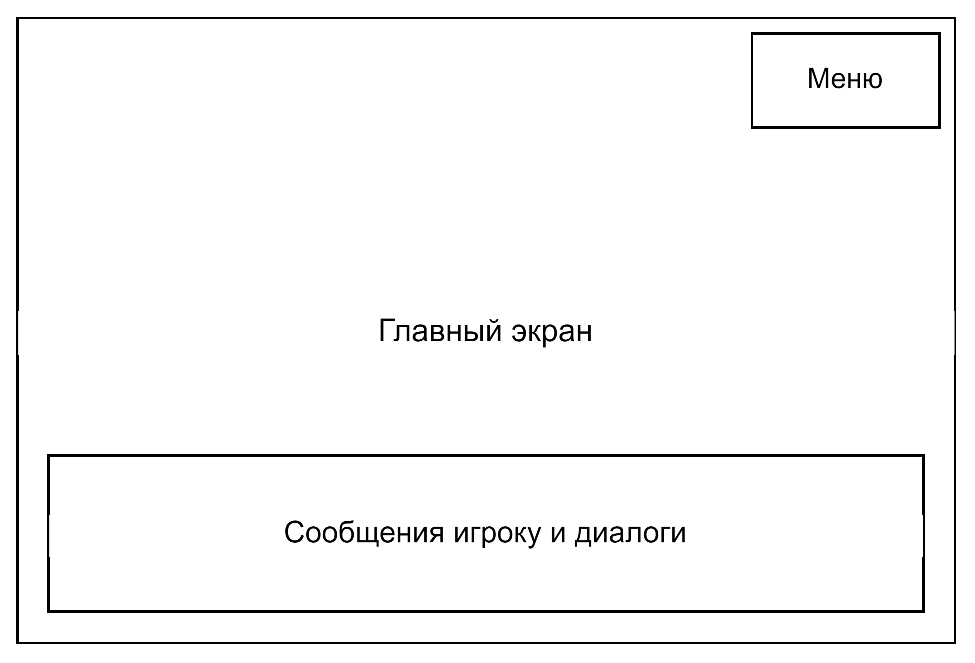
\includegraphics[width=1\linewidth]{maket}
\caption{Композиция шаблона интерфейса игры}
\label{maket:image}
\end{figure}
%\vspace{-\figureaboveskip} % двойной отступ не нужен (можно использовать, если раздел заканчивается картинкой)

\subsection{Правила игры}

Главный герой игры (ГГ) перемещается по локациям и выполняет квесты. Внутри каждой локации (кроме комнаты ГГ) имеется еще 2-3 подлокации. Начинается игра с предыстории в виде текста в диалоговой панели, который пользователь должен прочесть. Далее персонаж попадает в другие локации, перемещаясь по ним. Для того, чтобы пройти игру, нужно выполнить все квесты. Изначально не все локации доступны для посещения, а только те,что необходимы для текущего квеста. В игре присутствует цепочный механизм заданий, который предполагает последовательность действий (нельзя приступить к следующему заданию, не выполнив предыдущее).
Процесс выполнения квеста заключается в поиске определенных предметов, взаимодействии с персонажами, предметами и локациями игрового мира. Выполнив необходимые действия ГГ дальше двигается по квесту. Игрок может взаимодействовать с игровым миром с помощью компьютерной мыши. При наведении на активный объект курсор мыши поменяет состояние и по нему можно будет понять, с каким объектом мы имеем дело. Доступны следующие объекты взаимодействия с игроком:
\begin{enumerate}
\item Дверь – при наведении курсора иконка указателя меняется на уменьшенное изображение двери. При нажатии на дверь меняется локация.
\item Сущность – при наведении курсор меняется. При нажатии открывается диалог.
\item Предмет – при наведении на него курсор меняется на руку. При нажатии предмет исчезает с карты и появляется в инвентаре.
\item Переход на другую локацию – при наведении иконка курсора меняется на стрелку в направлении доступной локации, в которую хочет перейти пользователь.
\end{enumerate}
Инвентаря как такового нет. С ним нельзя взаимодействовать напрямую. Например, если при нажатии на какой-то объект требуется предмет в наличии у гг и его в инвентаре нет, то выйдет соответствующее сообщение, иначе – гг продвинется по квесту и получит другое сообщение.
По завершению финального квеста игры и прохождению всех локаций пользователь видит развязку сюжета, это конец игры.

\subsection{Сюжет игры}

Главная героиня засыпает и оказывается в одной из локаций игры – в лесу. Там ее пугает обиатель, и она решается выйти из сна, но у нее не получается. Тогда она начинает изучать лес и сталкиваясь с его обитателями, пытается узнать у них, как ей проснуться. Персонажи дают ей квесты, например, принести что-то или чем-то помочь. По выполнении очередного квеста она получает полезную информацию, предмет или пропуск на следующую локацию. В конце концов, она оказывается у хозяина этих земель, который должен ей помочь проснуться.После краткого диалога он убивает героиню, и она просыпается в кровати.

\subsection{Эпизод 1: Лес}

Оказываемся в сумеречном лесу и осмариваемся. Неподалеку видим призрака, подходим к нему и нажимаем для взаимодействия. Девочка подмечает, призрак достаточно милый и не страшный. Начинается диалог с призраком, по окончанию которого призрак моментально увеличивается в размерах и строит страшную гримасу. Девочка пугается и убегает на другую локацию внутри леса - кладбище. Также, она понимает, что у нее не получается выйти из сна. На кладбище видим статую плачущего ангела. Когда подходим к ней, слышим звуки плача. Нажимаем на призрака и в ходе диалога выясняется, что статуя потеряла очень важную вещь в лесу и не может ее найти, тк обездвижена. Взамен на эту вещь статуя обещает помочь выбраться из сна. Не найдя эту вещь в данной части леса, движемся в единственную доступную - начальную, где мы встретили призрака. Увидев призрака, девочка опять испугалась, но не убежала. При осмотре этой локации понимаем, что нужного нам предмета здесь нет, однако достаточно большую часть карты занимает огромный призрак, которого нужно как-то прогнать или уменьшить. Девочка не придумала ничего лучше, как напугать его. Кликаем по ней и смотрим, как она увеличивается в размерах и меняется в лице. Тем временем, по мере увеличения девочки, призрак уменьшается и в конце концов приходит в прежнюю милую форму, а вскоре и совсем убегает. Замечаем, что он закрывал собой тот самый предмет, который мы искали. Забираем его и приносим статуе. Та нас благодарит и говорит, что единственный, кто может помочь ей выбраться из сна - правитель этих земель, а дорогу к нему знает только лис, который спит в этом лесу. Нам открывается путь на следующую локаци этого леса - логово лиса. Зайдя на нее видим большую морду спящего животного. Для того чтобы его разбудить, нужно 3 раза нажать на него. Лис соглашается помочь девочке и провести ее к правителю, но взамен он просит помочь ему с его проблемой: в него что-то залезло и постоянно мешает жить. Лис предлагает девочке залесть к нему в пасть и посмотреть, что там. Нажимаем на пасть лиса и оказываемся в новой локации. Основные объекты и способы  взаимодействия с ними (при нажатии):
\begin{enumerate}
	\item Призрак - говорить.
	\item Статуя - говорить (получить квест), отдать предмет.
	\item Венок – взять, отдать статуе.
	\item Главный герой - вырасти и напугать призрака.
	\item Переход на другую локацию – перейти к призраку, статуе, лису или в пасть к лису.
	\item Лис - разбудить, говорить.
\end{enumerate}

\subsection{Интерфейс пользователя}

На основании анализа предметной области в программе должны быть реализованы следующие прецеденты:
\begin{enumerate}
\item Перемещение по локациям;
\item Перемещение персонажа по игровой области;
\item Просмотр кат-сцен;
\item Просмотр диалогов;
\item Взаимодействие с игровыми объектами при помощи компьютерной мыши.
\end{enumerate}
Таким образом, на рисунке ~\ref{prec:image}сформированы следующие действия пользователя и их последствия.
\begin{figure}[ht]
	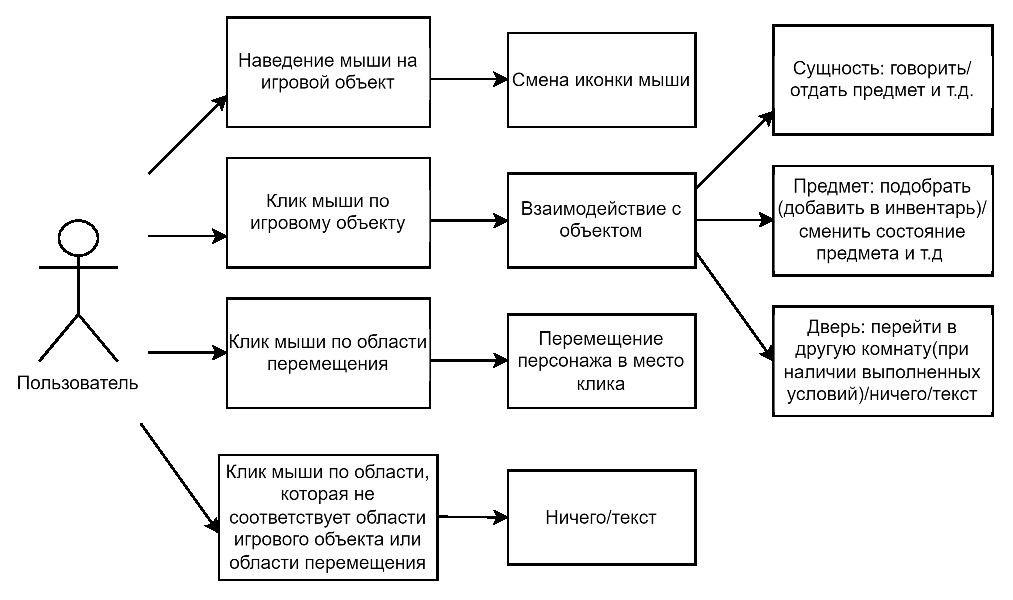
\includegraphics[width=1\linewidth]{prec}
	\caption{Шаблон интерфейса игры}
	\label{prec:image}
\end{figure}
%\vspace{-\figureaboveskip} % двойной отступ не нужен (можно использовать, если раздел заканчивается картинкой)

\subsection{Требования к оформлению документации}

Разработка программной документации и программного изделия должна производиться согласно ГОСТ 19.102-77 и ГОСТ 34.601-90. Единая система программной документации.

\section{Технический проект}
\subsection{Общая характеристика организации решения задачи}

Необходимо спроектировать и разработать приложение, которое должно способствовать продвижению компании на рынке.

Игровой движок -- базовое ПО компьютерной игры, которое пригодно для повторного использования и расширения, и тем самым может быть рассмотрено как основание для разработки множества различных игр без существенных изменений. В дополнение к многократно используемым программным компонентам, игровые движки предоставляют набор визуальных инструментов для разработки. Эти инструменты обычно составляют интегрированную среду разработки для упрощённой, быстрой разработки игр на манер поточного производства.

\subsection{Обоснование выбора технологии проектирования}

На сегодняшний день информационный рынок, поставляющий программные решения в выбранной сфере, предлагает множество продуктов, позволяющих достигнуть поставленной цели – разработки игрового приложения.

\subsubsection{Описание используемых технологий и языков программирования}

В процессе разработки игрового движка используются программные средства и языки программирования. Каждое программное средство и каждый язык программирования применяется для круга задач, при решении которых они необходимы.

\subsubsection{Язык программирования C\#}

C\# - объектно-ориентированный язык программирования общего назначения. Разработан в 1998—2001 годах группой инженеров компании Microsoft под руководством Андерса Хейлсберга и Скотта Вильтаумота как язык разработки приложений для платформы Microsoft .NET Framework и .NET Core. Впоследствии был стандартизирован как ECMA-334 и ISO/IEC 23270.
C\# относится к семье языков с C-подобным синтаксисом, из них его синтаксис наиболее близок к C++ и Java. Язык имеет статическую типизацию, поддерживает полиморфизм, перегрузку операторов (в том числе операторов явного и неявного приведения типа), делегаты, атрибуты, события, переменные, свойства, обобщённые типы и методы, итераторы, анонимные функции с поддержкой замыканий, LINQ, исключения, комментарии в формате XML.
На сегодняшний момент язык программирования C\# один из самых мощных, быстро развивающихся и востребованных языков в ИТ-отрасли. В настоящий момент на нем пишутся самые различные приложения: от небольших десктопных программок до крупных веб-порталов и веб-сервисов, обслуживающих ежедневно миллионы пользователей.
C\# является объектно-ориентированным и в этом плане много перенял у Java и С++. Например, C\# поддерживает полиморфизм, наследование, перегрузку операторов, статическую типизацию. Объектно-ориентированный подход позволяет решить задачи по построению крупных, но в тоже время гибких, масштабируемых и расширяемых приложений. И C\# продолжает активно развиваться, и с каждой новой версией появляется все больше интересных функциональностей.

\paragraph{Роль платформы .NET}

Когда говорят C\#, нередко имеют в виду технологии платформы .NET (Windows Forms, WPF, ASP.NET, .NET MAUI). И, наоборот, когда говорят .NET, нередко имеют в виду C\#. Однако, хотя эти понятия связаны, отождествлять их неверно. Язык C\# был создан специально для работы с фреймворком .NET, однако само понятие .NET несколько шире.
Фреймворк .NET представляет мощную платформу для создания приложений. Можно выделить следующие ее основные черты:
\begin{enumerate}
	\item Поддержка нескольких языков.
	\item Кроссплатформенность.
	\item Мощная библиотека классов.
	\item Разнообразие технологий.
	\item Производительность.
\end{enumerate}

\paragraph{Преимущества использования и изучения C\#}

C\# является управляемым языком программирования, что позволяет разработчику не следить за выделением и использованием памяти. Для этого существует CLR (Common Language Runtime) – виртуальная машина, которая занимается запуском приложения, а также управлением памятью.
Также C\# является строго типизированным и объектно ориентированным языком, что позволяет использовать ООП в его классическом виде. Здесь нет множественного наследования классов, что упрощает понимание ООП, но есть множественная реализация интерфейсов, что дает большую гибкость для разработчиков.
Большое сообщество и универсальность языка дают большое поле для деятельности. Как уже было указано ранее, вы можете разрабатывать веб-приложения, сложные микросервисные платформы, игры, а так же мобильные приложения. Здесь действительно серьезный инструментарий для разработки, такие IDE как Visual Studio или JetBrains Rider. Наличие огромнейшего разнообразия библиотек на все случаи жизни, от обратки изображений и видео, до нейросетей. А кроссплатформенность дает возможность писать код как на Windows, так и на macOS и Linux.
Как уже было сказано ранее, C\# является языком программирования общего назначения, а значит покрывает большое количество задач и областей, а именно:
\begin{enumerate}
	\item Web – разработка web-приложений и сервисов для платформ macOS, Windows, Linux и Docker.
	\item Mobile – разработка единой кодовой базы для построения нативных приложения для iOS и Android.
	\item Desktop – разработка нативных приложения под Windows и macOS.
	\item Microservices – разработка независимых компонентов запускаемы в Docker контейнерах.
	\item Cloud – использование существующих облачных решений или создание собственных. C\# поддерживается большинством облачных платформ, такими как Azure и AWS.
	\item Machine learning – разработка приложений искусственного интеллекта и машинного обучения, решающие проблемы машинного зрения, обработки речи, моделей предсказания, и тд.
	\item Game development – разработка 2D и 3D игра для самых популярных десктопных и мобильных платформ.
	\item Internet of Things (IoT) – разработка приложений для интернета вещей, имеющие поддержку Rasbery Pi и других одноплатных компьютеров.
\end{enumerate}

Исходя из вышеперечисленных областей применения видно, что платформа .NET и язык программирования C\# покрывают большой спектр проектов на рынке. Это говорит нам о том, что изучив язык программирования C\# с легкостью можно найти проект на любой вкус.

\paragraph{Описание движка}
AdventureGame - главный класс движка. Создается класс-наследник MyGame. Здесь будут храниться глобальные переменные конкретной игры (например флаги каких-то событий или квестов). Все функции движка там: добавить комнату, перейти в комнату, поместить персонажа/предмет, установить главного персонажа, удалить персонажа, предмет, запустить/остановить сценарий, передать управление в другой сценарий, разговор персонажа, взять предмет.
То есть это все то, что должно быть доступно в любом сценарии. Поэтому, надо делать класс AdventureGame статическим.Саму игру мы задаем в конструкторе это класса как множество комнат. 

Комната (Room) представляет собой совокупность объектов, а также хранит свою графику. Каждый объект может иметь свой небольшой управляющий сценарий. Эти сценарии работают параллельно, например, несколько объектов могут двигаться одновременно, или происходит одновременная анимация (качается дерево). В этих же сценариях можно управлять звуком (в будущем). Каждый сценарий запускается один раз и далее повторяется в цикле.Комната имеет отдельные сценарии для входа и выхода (то есть запускается один раз при входе героя в комнату и при выходе).К комнатам идет обращение по имени (задается при добавлении комнаты в движок).
Сценарий входа в комнату может проверять какие-то игровые ситуации и настраивать комнату перед отображением. Сценарий выхода может останавливать какие-то вещи.
Каждый объект в комнате имеет имя и сценарий по взаимодействию с ним по клику мыши (например открыть дверь).Также есть еще сценарий, когда герой пересекает объект (подходит к объекту). Здесь происходит перемещение персонажа в другую комнату (указывается в какую комнату). В другой комнате аналогично настроен сценарий на обратный проход (там другая дверь, другой объект).

Персонажи (Actor) имеют свою анимацию движения по комнате. По клику мыши в точку X,Y (или по программно заданным координатам) происходит автоматическое движение.
В комнате также задаются области (как множество прямоугольников), где происходит движение персонажей. Например, если в комнате в центре препятствие, то нужно 4 прямоугольника. Каждый прямоугольник должен касаться друг друга и не должен пересекаться с другими.
Каждый персонаж Actor может иметь набор предметов или инвентарь.

Текст добавляется методом SayLine (например в сценарии взаимодействия).
Объекты расставляются в комнате по координатам. При взаимодействии с объектом персонаж находится в определенном месте (эта позиция задается для объекта) - например, с левой стороны двери. Состояние персонажа (куда он смотрит после того как подошел в заданную позицию) задается в сценарии взаимодействия (запускается после того как персонаж пришел в заданную позицию).
Объект может иметь несколько состояний (одно минимум). Каждое состояние сопоставлено с о спрайтом или анимацией. Например, закрытая и открытая дверь.
Взять объект - PickUpObject - объект попадает в хранилище персонажа.

Анимацию задаем как последовательность кадров с заданной скоростью.
Автоматическое движение объекта задаем в сценарии.

Сценарий запускается (StartScript), и затем работает до тех пор пока не будет остановлен (StopScript).
В сценарии задаем шаги движения, между которыми вызываем Yield (передать управление другому потоку). То есть сценарии - это параллельные потоки.
Глобальные переменные могут быть в классе конкретной игры или в статическом классе Globals. Чтобы к ним обратиться, функция сценария должна также быть в классе игры. Локальные переменные могут быть внутри конкретной комнаты, тогда локальные сценарии находятся в классе комнаты.

Сценарий - это любой метод (например у MyGame или у конкретной комнаты (класса, потомка от Room).
То есть мы в движок передаем метод (через делегат), а уже сам движок делает все что нужно (запускает поток).
У наследника указываются только свои поля. Сценарии размещаются в зависимости от того, что там делается.
Если просто перемещение, смена состояния, смена комнаты - тогда в классе конкретной комнаты (потомка Room).

Отрисовка всех объектов происходит с помощью таймера и события Form\_Paint. Таймер обращается к GraphicsManager, который меняет состояние объектов когда это нужно. Это происходит каждый тик таймера. Затем событие Form\_Paint с помощью Graphics отображает измененные объекты на форме. На выходе мы получаем актуальное состояние каждого объекта, которое можем наблюдать в реальном времени. Это может быть анимация перемещения, появления или исчезновения объекта.


\subsection{Диаграмма компонентов классов}

Диаграмма компонентов описывает особенности физического представления разрабатываемой системы. Она позволяет определить архитектуру системы, установив зависимости между программными компонентами, в роли которых может выступать как исходный, так и исполняемый код. Основными графическими элементами диаграммы компонентов являются компоненты, интерфейсы, а также зависимости между ними. На рисунке \ref{diagram:image} изображена диаграмма компонентов для проектируемой системы. Она включает в себя основной класс движка игры AdventureGame и производные от него классы, класс Object с наследниками и их параметрами (полями и методами).

\begin{figure}[ht]
\center{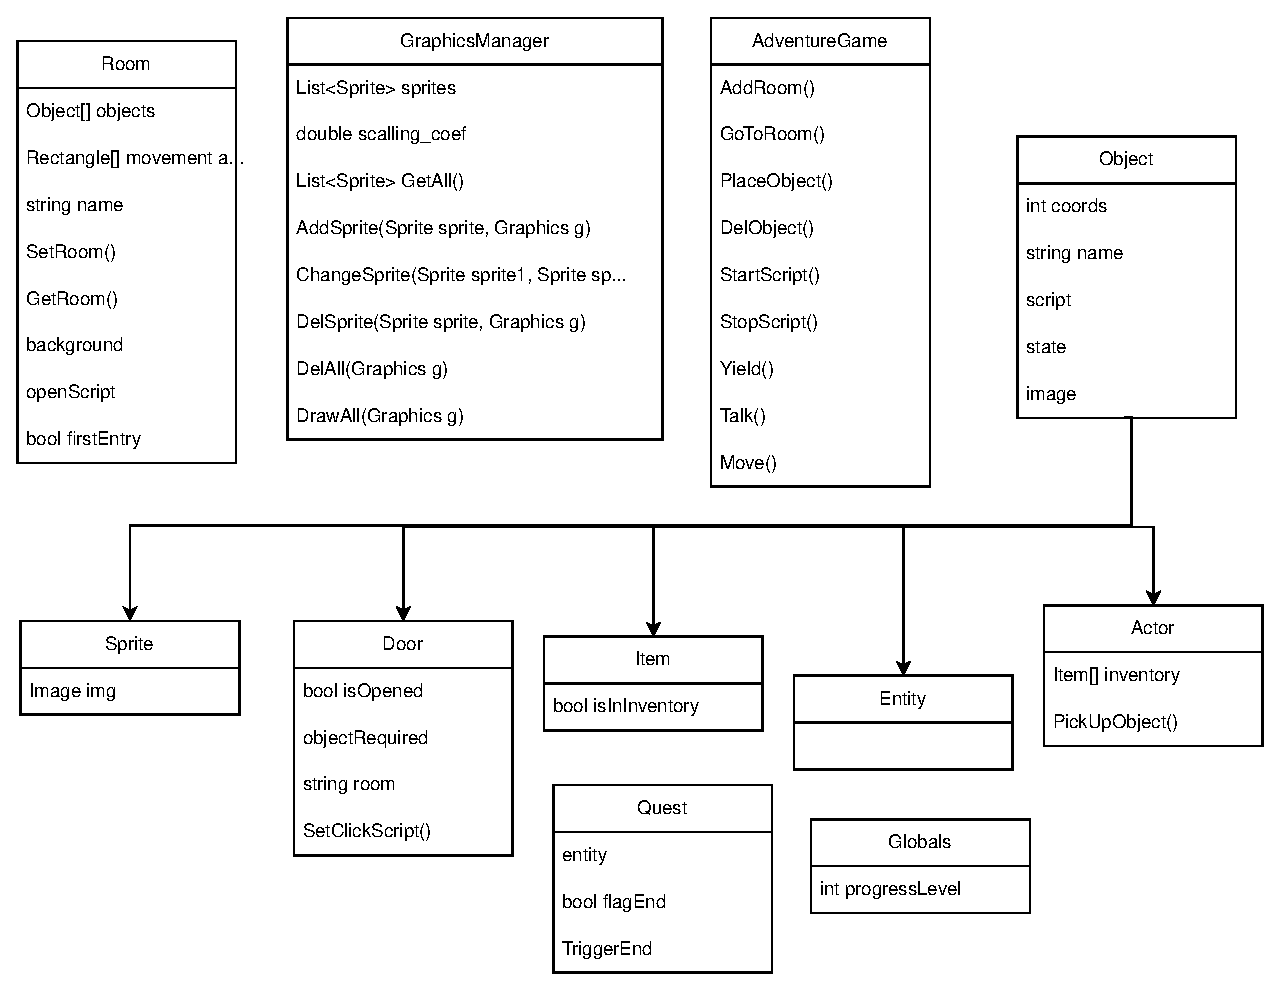
\includegraphics[width=1\linewidth]{diagram}}
\caption{Диаграмма компонентов}
\label{diagram:image}
\end{figure}

\subsection{Описание классов}

\begin{enumerate}
	\item[GraphicsManager] - класс, управляющий спрайтами. Содержит в себе:
	\begin{itemize}
		\item List<Sprite> sprites - список спрайтов;
		\item double scalling\_coef - коэффициент приближения;
		\item AddSprite(Sprite sprite, int x, int y) - добавляет в список спрайт, сохраняет координаты;
		\item ChangeSprite(Sprite sprite1, Sprite sprite2) - меняет местами спрайты в списке;
		\item DelSprite(Sprite sprite) - удаляет спрайт из списка;
		\item DelAll() - очищает список спрайтов;
		\item UpdateGraphics(Graphics g) - с помощью Graphics добавляет все спрайты из списка на форму.
	\end{itemize}
	\item[Sprite] - класс, хранящий в себе изображения игровых объектов Image img.
	\item[Object] - абстрактный класс, от которого наследуются классы Sprite, Item, Entity, Actor, Door.
	\item[Entity] - класс сущностей. Потомок класса Object. Сущность - игровой объект, который считается одушевленным, то есть с ним можно поговорить и нельзя подобрать в инвентарь, в отличие от объекта Item.
	\item[Item] - класс предметов. Предмет - это игровой объект, который является неодушевленным, то есть вещью, которую можно взять в инвентарь. С вещью нельзя разговаривать, в отличие от объекта класса Entity, но она также является потомком класса Object.
	\item[Actor] - главный персонаж игры, которым управляет пользователь. Именно он находится в центре сюжета. Является наследником Object, так как имеет схожие свойства.
	\item[Door] - еще один наследник класса Object. Является по своей сути объектом, реализующим переход между комнатами(Room).
	\begin{itemize}
		\item bool isOpened - состояние двери (открыта/закрыта);
		\item objectRequired - условия, необходимые для того, чтобы дверь открылась. Проверяются при нажатии на дверь;
		\item string name - название комнаты, в которую ведет дверь;
		\item SetClickScript() - события, которые произойдут, когда польователь кликнет на дверь;
	\end{itemize}
	\item[Room] - комната(подлокация), в которой происходит сюжетное действие и игровой процесс. Содержит следующие поля и методы:
	\begin{itemize}
		\item Object[] objects - список всех объектов, которые размещены в данной комнате;
		\item Rectangle[] moveArea - область, по которой может перемещаться персонаж (Actor). Определяется набором прямоугольников, которые не должны пересекаться;
		\item string name - название комнаты;
		\item bool firstEntry - показывает, находится ли персонаж в данной комнате впервые;
		\item SetRoom(string roomName) - устанавливает комнату со всеми ее объектами и их состояниями;
		\item GetRoom(string roomName) - получает комнату со всеми ее объектами и их состояниями;
	\end{itemize}
	\item[Globals] - в данном классе находятся глобальные переменные (флаги) текущей игры. Например, int progressLevel в виде простого числа показывает прогресс игрока в игре.
	\item[AdventureGame] - абстрактный класс, управляющий игрой. Имеет следующие методы:
	\begin{itemize}
		\item AddRoom(string roomName) - добавить комнату;
		\item GoToRoom(string roomNAme) - перейти в комнату;
		\item PlaceObject(Object object, int x, int y) - поместить объект на карту по координатам x и y;
		\item DelObject(Object object) - удалить объект;
		\item StartScript(???) - запускает скрипт;
		\item StopScript(???) - останавливает скрипт;
		\item Yeild(???) - передает управление другому скрипту;
		\item Talk(???) - говорить с персонажем. Отображает текст в текстовом поле внизу экрана. 
		\item Move() - перемещение объектов.
	\end{itemize}
\end{enumerate}




\ifПрактика{}\else{
   \section{Рабочий проект}
\subsection{Классы, используемые при разработке сайта}

Можно выделить следующий список классов и их методов, использованных при разработке web-приложения (таблица \ref{class:table}). Пример таблицы с уменьшенным межстрочным интервалом.

\renewcommand{\arraystretch}{0.8} % уменьшение расстояний до сетки таблицы
\begin{xltabular}{\textwidth}{|X|p{2.5cm}|>{\setlength{\baselineskip}{0.7\baselineskip}}p{4.85cm}|>{\setlength{\baselineskip}{0.7\baselineskip}}p{4.85cm}|}
\caption{Описание классов Bitrix, используемых в приложении\label{class:table}}\\
\hline \centrow \setlength{\baselineskip}{0.7\baselineskip} Название класса & \centrow \setlength{\baselineskip}{0.7\baselineskip} Модуль, к которому относится класс & \centrow Описание класса & \centrow Методы \\
\hline \centrow 1 & \centrow 2 & \centrow 3 & \centrow 4\\ \hline
\endfirsthead
\caption*{Продолжение таблицы \ref{class:table}}\\
\hline \centrow 1 & \centrow 2 & \centrow 3 & \centrow 4\\ \hline
\finishhead
CMain & Главный модуль & CMain – главный класс страницы web-приложения. После одного из этапов по загрузке страницы в сценарии становится доступным инициализированный системой объект данного класса с именем \$APPLICATION & void ShowTitle(string property\_code = «title», bool strip\_tags = true)
Выводит заголовок страницы
void SetTitle(string title)
Устанавливает заголовок страницы

void ShowCSS(bool external = true, bool XhtmlStyle = true)
Выводит таблицу стилей CSS страницы\\
\hline CFile & Главный модуль & CFile – Класс для работы с файлами и изображениями & array GetFileArray (int file\_id)
Метод возвращает массив, содержащий описание файла (путь к файлу, имя файла, размер) с идентификатором file\_id
\end{xltabular}
\renewcommand{\arraystretch}{1.0} % восстановление сетки

\subsection{Модульное тестирование разработанного web-сайта}

Модульный тест для класса User из модели данных представлен на рисунке \ref{unitUser:image}.

\begin{figure}[ht]
\begin{lstlisting}[language=Python]
from django.test import TestCase
from .models import *
User = get_user_model()


class ShpoTestCases(TestCase):

    def setUp(self) -> None:
        self.user = User.objects.create(username='testtestovich', password='testtestovich', first_name='Sad', last_name='')

    def test_2(self):

        self.assertEqual(self.user.first_name, 'Sad')
        self.assertEqual(self.user.last_name, 'Cat')
        print((self.user))
        print((self.user.first_name))
        print((self.user.last_name))
\end{lstlisting}  
\caption{Модульный тест класса User}
\label{unitUser:image}
\end{figure}

\subsection{Системное тестирование разработанного web-сайта}

На рисунке \ref{main:image} представлена главная страница сайта «Русатом – Аддитивные технологии».
\newpage % при необходимости можно переносить рисунок на новую страницу
\begin{figure}[H] % H - рисунок обязательно здесь, или переносится, оставляя пустоту
\center{\includegraphics[width=1\linewidth]{main1}}
\center{\includegraphics[width=1\linewidth]{main2}}
\center{\includegraphics[width=1\linewidth]{main3}}
\caption{Главная страница сайта «Русатом – Аддитивные технологии»}
\label{main:image}
\end{figure}

На рисунке \ref{menu:image} представлен динамический вывод заголовков, включающий в себя искомые фразы при поиске фраз.

\begin{figure}[ht]
\center{\includegraphics[width=1\linewidth]{menu}}
\caption{Динамический вывод заголовков}
\label{menu:image}
\end{figure}

На рисунке \ref{enter:image} представлен ввод данных для публикации новости.

\begin{figure}[ht]
\center{\includegraphics[width=1\linewidth]{enter}}
\caption{Ввод данных для публикации очень-очень длинной, интересной и полезной новости}
\label{enter:image}
\end{figure}

   \section*{ЗАКЛЮЧЕНИЕ}
\addcontentsline{toc}{section}{ЗАКЛЮЧЕНИЕ}

Преимущества аддитивных технологий заключается в разнообразии процессов, позволяющих применять их в различных областях производства. Существенным ограничением же является и экономическая составляющая, которая не позволит внедрить аддитивное производство повсеместно.
  
Компании, видя, как развиваются информационные технологии, пытаются использовать их выгодно для своего бизнеса, запуская свой сайт для того, чтобы заявить о своем существовании, проинформировать потенциального клиента об услугах или продуктах, которые предоставляет. 
Для продвижения компании «Русатом – Аддитивные технологии» был разработан веб-сайт на основе системы «1С-Битрикс: Управление сайтом».

Основные результаты работы:

\begin{enumerate}
\item Проведен анализ предметной области. Выявлена необходимость использовать 1С-Битрикс.
\item Разработана концептуальная модель web-сайта. Разработана модель данных системы. Определены требования к системе.
\item Осуществлено проектирование web-сайта. Разработана архитектура серверной части. Разработан пользовательский интерфейс web-сайта.
\item Реализован и протестирован web-сайт. Проведено модульное и системное тестирование.
\end{enumerate}

Все требования, объявленные в техническом задании, были полностью реализованы, все задачи, поставленные в начале разработки проекта, были также решены.

Готовый рабочий проект представлен адаптивной версткой сайта. Сайт находится в публичном доступе, поскольку опубликован в сети Интернет.  

}\fi
\addcontentsline{toc}{section}{СПИСОК ИСПОЛЬЗОВАННЫХ ИСТОЧНИКОВ}

\begin{thebibliography}{9}

    \bibitem{javascript} Вигерс, К. Разработка требований к программному обеспечению / К. Вигерс. – Санкт-Петербург~: Вигерс, 2020. – 736 с. – ISBN 978-5-9775-3348-5. – Текст~: непосредственный.
    \bibitem{php} Космин, В. Основы научных исследований : учебное пособие / В. Космин. – Москва, 2020. – 238 с. – ISBN 978-5-369-01753-1. – Текст~: непосредственный.
    \bibitem{css} Рихтер, Д. Программирование на платформе Microsoft.NET. Framework 4.5 на языке C\# / Д. Рихтер. – Санкт-Петербург : Питер, 2017. – 896 с. – ISBN 978-5-496-00433-6. – Текст~: непосредственный.
    \bibitem{mysql}	Фаулер, Рефакторинг. Улучшение существующего кода / М. Фаулер. – Москва~: НТ Пресс, 2013. – 432 с. – ISBN 978-5-477-01174-2. – Текст~: непосредственный.
	\bibitem{html5}	Сидоренко, И. Дизайнер интерфейсов / И.	Сидоренко – Москва~: Вильямс, 2012. – 368 с. – ISBN 978-5-699-57580-0. – Текст~: непосредственный.
	\bibitem{htmlcss}	Хейлсберг, А. Язык программирования C\# / А. Хейлсберг. – Питер~: Эксмо, 2014. – 773 с. – ISBN 978-5-699-64193-2. – Текст~: непосредственный.
	\bibitem{bigbook}	Макфарланд, Д. Большая книга CSS / Д. Макфарланд. – Санкт-Петербург : Питер, 2012. – 560 с. – ISBN 978-5-496-02080-0. – Текст~: непосредственный.
	\bibitem{uchiru}	Лоусон, Б. Изучаем HTML5. Библиотека специалиста / Б. Лоусон, Р. Шарп. – Санкт-Петербург : Питер, 2013 – 286 с. – ISBN 978-5-459-01156-2. – Текст~: непосредственный.
	\bibitem{chaynik}	Мартин, Р. Чистая архитектура. Искусство разработки программного обеспечения / Р. Мартин – Санкт-Петербург : Питер, 2018 – 352 с. – ISBN 978-5-4461-0772-8. – Текст~: непосредственный.    
	\bibitem{22}	Титтел, Э. HTML5 и CSS3 для чайников / Э. Титтел, К. Минник. – Москва~: Вильямс, 2016 – 400 с. – ISBN 978-1-118-65720-1. – Текст~: непосредственный.    
	\bibitem{1231}	Белик, А. Г. Проектирование и архитектура программных систем / А. Г.  Белик, В. Н. Цыганенко. – Омск~: ОмГТУ, 2016 – 96 с. – ISBN 978-5-8149-2258-8. – Текст~: непосредственный.	
	\bibitem{htmlcss}	Хейлсберг, А. Язык программирования C\# / А. Хейлсберг. – Питер~: Эксмо, 2014. – 773 с. – ISBN 978-5-699-64193-2. – Текст~: непосредственный.
\end{thebibliography}

\ifВКР{\appendix{Представление графического материала}

Графический материал, выполненный на отдельных листах,
изображен на рисунках А.1--А.\arabic{числоПлакатов}.
\setcounter{числоПлакатов}{0}

\renewcommand{\thefigure}{А.\arabic{figure}} % шаблон номера для плакатов

\begin{landscape}

\begin{плакат}
    
\includegraphics[width=0.82\linewidth]{плакат1.png}
    \заголовок{Сведения о ВКРБ}
    \label{pl1:image}      
\end{плакат}

\begin{плакат}
    
\includegraphics[width=0.82\linewidth]{плакат2.png}
    \заголовок{Цель и задачи разработки}
    \label{pl2:image}      
\end{плакат}

\begin{плакат}
    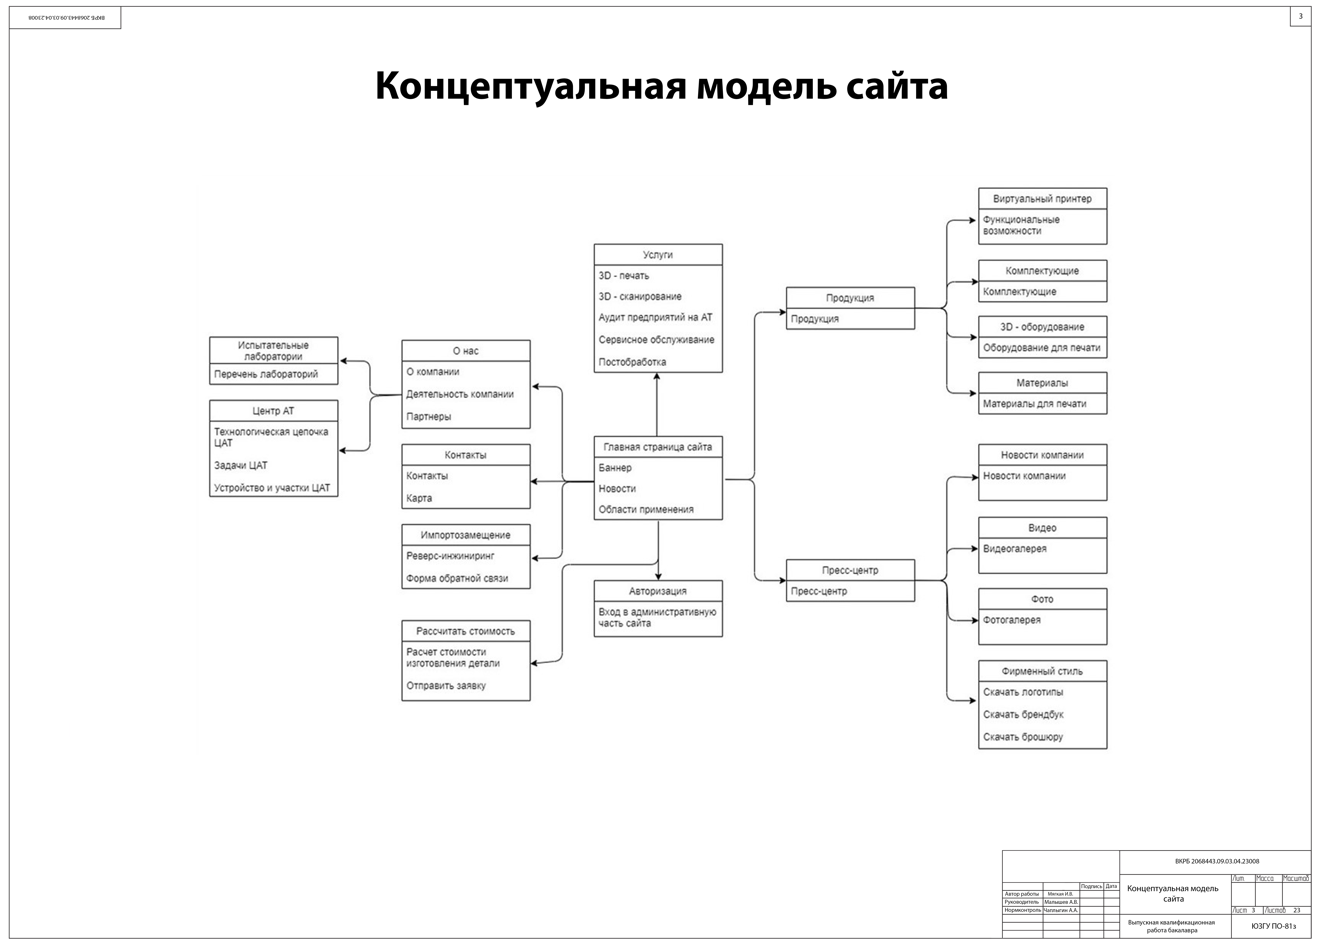
\includegraphics[width=0.82\linewidth]{плакат3.png}
    \заголовок{Концептуальная модель сайта}
    \label{pl3:image}      
\end{плакат}

\begin{плакат}
    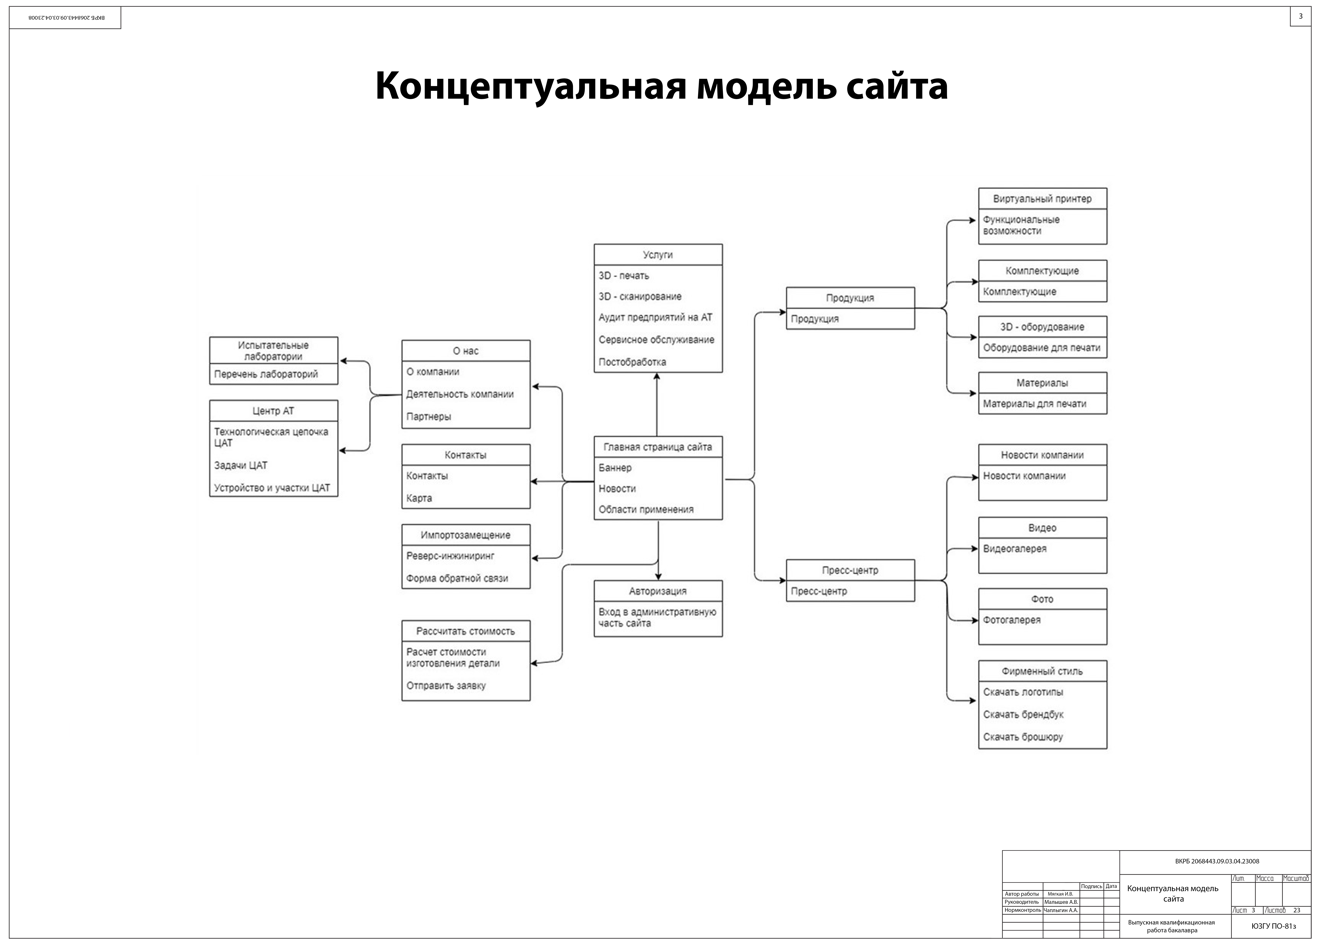
\includegraphics[width=0.82\linewidth]{плакат3.png}
    \заголовок{Еще плакат}
    \label{pl4:image}      
\end{плакат}

\end{landscape}
}\fi
\ifПрактика{}\else{\appendix{Фрагменты исходного кода программы}

main.tex
\lstinputlisting[language=Tex, frame=none]{main.tex}

ТехПроект.tex
\lstinputlisting[language=Tex, frame=none]{ТехПроект.tex}

\ifВКР{
\newpage
\addcontentsline{toc}{section}{На отдельных листах (CD-RW в прикрепленном конверте)}
\begin{center}
\textbf{Место для диска}
\end{center}
}\fi
}\fi
\end{document}
